On note $a = BC$, $b = CA$, $c = AB$ les côtés d'un triangle $ABC$ et
$\mathcal{S}$ son aire. On veut démontrer l'inégalité de Weitzenböck
(1919, posée à l'OIM 1961) :
\[
a^2 + b^2 + c^2 \geqslant 4\sqrt{3}\,\mathcal{S},
\]
avec égalité si et seulement si le triangle est équilatéral.

\emph{Idée directrice :} on mesure l'écart entre le triangle $ABC$ et le
triangle équilatéral $ABC'$ construit sur $[AB]$, du même côté que $C$
(en pointillés).

\begin{center}
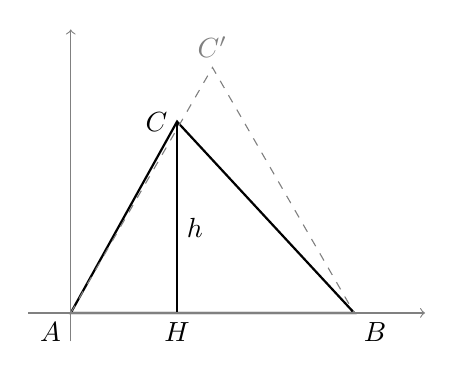
\begin{tikzpicture}[scale=0.9]
  \coordinate (A) at (0,0);
  \coordinate (B) at (4,0);
  \coordinate (C) at (1.5,2.7);
  \coordinate (E) at (2,3.464);
  \coordinate (H) at (1.5,0);
  \draw[thick] (A) -- (B) -- (C) -- cycle;
  \draw[dashed,gray] (A) -- (E) -- (B);
  \draw (C) -- (H);
  \draw[->,gray] (-0.6,0) -- (5,0);
  \draw[->,gray] (0,-0.4) -- (0,4);
  \node[below left] at (A) {$A$};
  \node[below right] at (B) {$B$};
  \node[left] at (C) {$C$};
  \node[above,gray] at (E) {$C'$};
  \node[below] at (H) {$H$};
  \node[right] at (1.5,1.2) {$h$};
\end{tikzpicture}
\end{center}

\begin{enumerate}
  \item On place le triangle dans un repère orthonormé avec $A(0\,;0)$,
  $B(c\,;0)$ et $C$ dans le demi-plan $y > 0$. Justifier qu'on peut écrire
  $C\left(\frac{c}{2} - x\,;\,h\right)$ avec $x \in \mathbb{R}$ et $h > 0$,
  puis exprimer $a^2$, $b^2$ et $\mathcal{S}$ en fonction de $c$, $x$ et $h$.
  \item Quelles valeurs de $x$ et $h$ correspondent au triangle équilatéral ?
  On pose $y = h - \frac{\sqrt{3}}{2}\,c$ (écart de hauteur).
  \item Montrer que
  \[
  a^2 + b^2 + c^2 - 4\sqrt{3}\,\mathcal{S} = 2x^2 + 2y^2.
  \]
  (Indication : regrouper les termes en $h$ et compléter le carré.)
  \item Conclure, et déterminer le cas d'égalité.
  \item Vérifier l'inégalité sur le triangle de côtés $3$, $4$, $5$.
\end{enumerate}
